\section{Introduction}

\begin{frame}{Motivation}
Emerging Requirements :
\begin{itemize}
\item Instantaneous Encryption 
\item Computation of ciphertext with a single clock cycle
\item Low Latency
\item Low hardware costs 
\item Low space and time overhead
\end{itemize}
PRINCE Cipher Fulfils all these requirements  
\end{frame}

\begin{frame}{Salient features}
\begin{itemize}
\item Inspired From the FX construction 
\item SPN Based 
\item Inspired from PRESENT (Another Lightweight cipher)
\item Balance between Speed/Efficiency and Security 
\item Considerably Less Area (In terms of gates) Than PRESENT-80 and AES-128 
\item The Same Core function works both in encryption and decryption (No need of Additional Logic gates)
\end{itemize}

\end{frame}

\begin{frame}{Contruction}
The FX-Construction is built using a core function and 2 whitening keys which are used in pre-processing and post-processing \\ \\ 
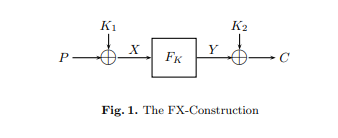
\includegraphics[]{FX.PNG}
\end{frame}